% Article template for Mathematics Magazine
% Revised 7/2002  Thanks for Greg St. George
\documentclass[12pt]{article}
\usepackage{amssymb}
\usepackage[ngerman]{babel}
\usepackage[utf8]{inputenc}
\usepackage{amsmath}
\usepackage{pf2}
\usepackage{graphicx}
\renewcommand{\baselinestretch}{1.2}
%This is the command that spaces the manuscript for easy reading
\newtheorem{zeige}{Zeige}


%todo 
\usepackage[colorinlistoftodos,prependcaption,textsize=tiny]{todonotes}
\usepackage{xargs}                      % Use more than one optional parameter in a new commands
\newcommandx{\QUESTION}[2][1=]{\todo[linecolor=none,backgroundcolor=blue!15,bordercolor=none,#1]{\textbf{QUESTION: }#2}}

\pflongnumbers



\begin{document}
%\thispagestyle{empty}
\begin{center}
\Large
% TITLE GOES HERE
Logik und Komplexität  \textsc{ Übung 7 }
\end{center}

\begin{flushright}
Denis Erfurt, 532437\\
HU Berlin \\

\vspace{2 mm}

\end{flushright}

\subsection*{Aufgabe 1)}
\subsubsection*{a)}

\textbf{zeige} Conn ist nicht $L_{\infty \omega}^2$-definierbar in UGraph \\
nach Theorem 4.24 genügt e zu zeigen, dass es ein $\mathfrak{A}\in Conn$ und 
ein $\mathfrak{B}\in UGraph \setminus Conn$ gibt, so dass 
$\mathfrak{A}\approx^2_\infty \mathfrak{B}$ \\
Sei $\mathfrak{A} := K_8$ ein Kreis mit 8 Steinen, 
$\mathfrak{B}:=K_4\cup K_4$ 2 Kreise mit jeweils 4 Steinen \\
\textbf{zeige } $\mathfrak{A}\approx^2_\infty \mathfrak{B}$\\
\textbf{IA: } Für alle Steine gilt: $a_i,b_i = *$. Insbesondere sind
die Gewinnbedingungen für Duplicator erfüllt.
\textbf{IS: } $i \rightarrow  i+1$\\

O.b.d.A bewegt Spoiler den Stein $\alpha_k$ von $a_k\in A$ nach $a_{k'}\in A$,
die Fälle für B sind analog.

Sei $k,l\in \{1,2\}$ sowie $k\neq l$.

\textbf{Fall 1.} In Runde i+1 gilt: $\alpha_k = \alpha_l$ \\
So setzt Duplicator $\beta_k$ auf $\beta_l$ und Gewinnt in Runde i+1\\

\textbf{Fall 2.} In Runde i+1 gilt: $(\alpha_k, \alpha_l) \in E^\mathfrak{A}$\\

\[ \phi := \forall x_1 \exists x_2 \exists x_3 ( \neg x_2 = x_3 ) \land E(x_1,x_2) \land E(x_1,x_3) \] 

Beobachhtung 1: $ \mathfrak{B} \models \phi$

\textbf{Fall 2.1.} In Runde i war $(\alpha_k, \alpha_l) \in E^\mathfrak{A}$
    
    Nach Beobachhtung 1. gibt es ein $b_{k'} \in B$ mit $b_k \neq b_{k'}$ und 
    $(b_{k'}, \beta_l)\in E^\mathfrak{B}$.
    
    Duplicator wählt $\beta = b_{k'}$ und gewinnt die Runde i+1.
    
  \textbf{Fall 2.2.} In Runde i war $(\alpha_k, \alpha_l) \notin E^\mathfrak{A}$
    
    Nach Beobachhtung 1. gibt es ein $b_{k'} \in B$ mit $(b_{k'}, \beta_l)\in E^\mathfrak{B}$.
    
    Duplicator wählt $\beta = b_{k'}$ und gewinnt die Runde i+1.
    
\textbf{Fall 3.} In runde i+1 gilt: $(\alpha_k, \alpha_l) \notin E^\mathfrak{A}$\\
    
  \textbf{Fall 3.1.} Spoiler wählt $\alpha_k = *$
    
    Duplicator wählt $\beta_k = *$ und gewinnt die Runde i+1.
    
  \textbf{Fall 3.2.} Spoiler wählt ein beliebiges $a_{k'}$
    
    Duplicator wählt ein beliebiges $\beta_k = b_{k'}$ so dass $(b_{k'},b_l)\notin E^\mathfrak{B}$ und gewinnt die Runde i+1.
    

    Damit ist gezeigt, dass Duplicator die Runde i+1 übersteht. Somit hat Duplicator
    eine Gewinnstrategie im 2-Pebble-Spiel.
    
    \qed
    

\subsubsection*{b)}
% \textbf{Behauptung}: Conn ist nicht $L_{\infty \omega}^\omega$-definierbar in UGraphs.
%
% Nach Theorem 4.24. genügt es zu Zeigen, dass für jedes $n\in \mathbb{N}$ ein
% $\mathfrak{A}_n\in Conn$ und $\mathfrak{B}_n\in UGraphs \setminus Conn$ gibt,
% so dass gilt: $\mathfrak{A}_n \approx_\infty^n \mathfrak{B}_n$.
%
% Sei $G_r$ ein Gitterstruktur mit $r^2$ Knoten.
%
% Sei $\mathfrak{A}_n:= G_n$ und $\mathfrak{B}_n := G_n \cup G_n$. \\
% Offensichtlich ist $\mathfrak{A}_n \in Conn$ und $\mathfrak{B}_n \in UGraphs\setminus Conn$.\\
%
% \textbf{z.Z.: $\mathfrak{A}_n \approx_\infty^n \mathfrak{B}_n$}

Behauptung: Conn ist $L^3_{\infty \omega}$-definierbar in UGraph.

Sei $\mathfrak{A} \in Conn$ sowie $\mathfrak{B}\in UGraphs \setminus Conn$.\\
Sei $\mathfrak{B}:=\mathfrak{B}_1\cup \mathfrak{B}_2$.

nach Theorem 4.24. genügt es zu zeigen, dass Spoiler eine Gewinnstrategie für 
beliebige $\mathfrak{A}$ und $\mathfrak{B}$ besitzt: Spoiler wählt $\beta_1, \beta_2
\in B_1$ und $\beta_3\in B_2$ um zu gewinnen muss Duplicator 
$\alpha_1,\alpha_2,\alpha_3 \in A$ wählen. Nun wählt in Runde i+1 Spoiler das 
$\alpha_i$ mit $i\in \{1,2\}$ aus, welches die größte Entfernung zum $\alpha_3$ besitzt und plaziert es
auf das $a\in A$, welches die geringste Entfernung zum $\alpha_3$ besitzt und
noch eine Verbindung zum $\alpha_j$ mit $j\in \{1,2\}\setminus \{i\}$ besitzt. 
Die Distanz zwischen den $\alpha_1,\alpha_2$ Steinen und dem $\alpha_3$ Stein verringert 
sich bei jeder Runde um 1.
Um zu gewinnen muss Duplicator einen Stein in $B_1$ bewegen. Nach endlich vielen
Runden ist besitzt ein $\alpha_i$ eine Verbindung mit $\alpha_j$ sowie $\alpha_3$.
Da jedoch $\beta_1$ sowie $\beta_2$ sich auf Steinen in $B_1$ befinden kann Duplicator
keine Verbindung zwischen den 3 Steinen herstellen. Somit ist es kein partialler Isomorphismus und Duplicator hat nach endlich vielen Zügen verlohren.


\subsection*{Aufgabe 2)}

\subsubsection*{a)}

\[ \varphi_1(x) := \forall y E(x,y) \] 

\begin{proof}
  \step{<1>1} { \prove{ $\varphi_1$ ist keine um x lokale Formel. } }
  \step{<1>2} { \pflet{ $\sigma := \{E\}$} }
  \step{<1>3} { \pflet{ $\mathfrak{A} := (\{1,2\},\{\})$} }
  \step{<1>4} { $\mathfrak{A}\nvDash \varphi_1[1]$ }
  \step{<1>5} { Für alle $r\in \mathbb{N}$ gilt: $\mathcal{N}_r^\mathfrak{A} (1) = (\{1\},\{\})$ }
  \step{<1>6} { $\mathcal{N}_r^\mathfrak{A}[1] \models \varphi_1[1]$ }
  \qedstep 
  \begin{proof}
    \pf Def. 5.3. b), \stepref{<1>4}, \stepref{<1>6}
  \end{proof}
\end{proof}

\paragraph{GNF:}
\[ \varphi_1^{Nr(x)}(x) := ( \forall y\ dist(x,y) \leq 2 \rightarrow E(x,y) ) 
  \land ( \neg \exists z_1 \exists z_2\ dist(z_1,z_2) > 2 )  
\] 


\subsubsection*{b)}

\[ \varphi_2(x_1,x_2) := \neg x_1=x_2 \land \forall y E(x_1,y) \lor E(x_2,y) \] 

\begin{proof}
  \step{<1>1} {\prove{ $\varphi_2$ ist  keine um $x_1, x_2$ lokale Formel. }}
  \step{<1>2} {\pflet{ $\sigma := \{E\}$ }}
  \step{<1>3} {\pflet{ $\mathfrak{A} := (\{1,2,3\},\{(1,2),(2,1)\})$ }}
  \step{<1>4} {$\mathfrak{A} \nvDash \varphi_2[1,2]$}
  \step{<1>5} { Für alle $r\in \mathbb{N}$ gilt: $\mathcal{N}_r^\mathfrak{A} (1,2) = 
    (\{1,2\},\{(1,2),(2,1)\})$ }
  \step{<1>6} {$\mathcal{N}_r^\mathfrak{A}(1,2) \models \varphi_2[1,2]$}
  \qedstep 
  \begin{proof}
    \pf Def. 5.3. b), \stepref{<1>4}, \stepref{<1>6}
  \end{proof}
\end{proof}

\paragraph{GNF:}

\begin{eqnarray}
  \varphi_2(x_1,x_2) &:= &\neg x_1=x_2 \\ 
  && \land ( \forall y\ dist(y, \{x_1, x_2\})\leq 2 \rightarrow E(x_1,y) \lor E(x_2,y) ) \\ 
  && \land \neg \exists z_1 \exists z_2 \exists z_3 ( \bigwedge_{z_i\neq z_j}\ dist(z_i,z_j) > 2 )
\end{eqnarray}


\subsection*{Aufgabe 3)}

\begin{figure}[h]
 \centering
 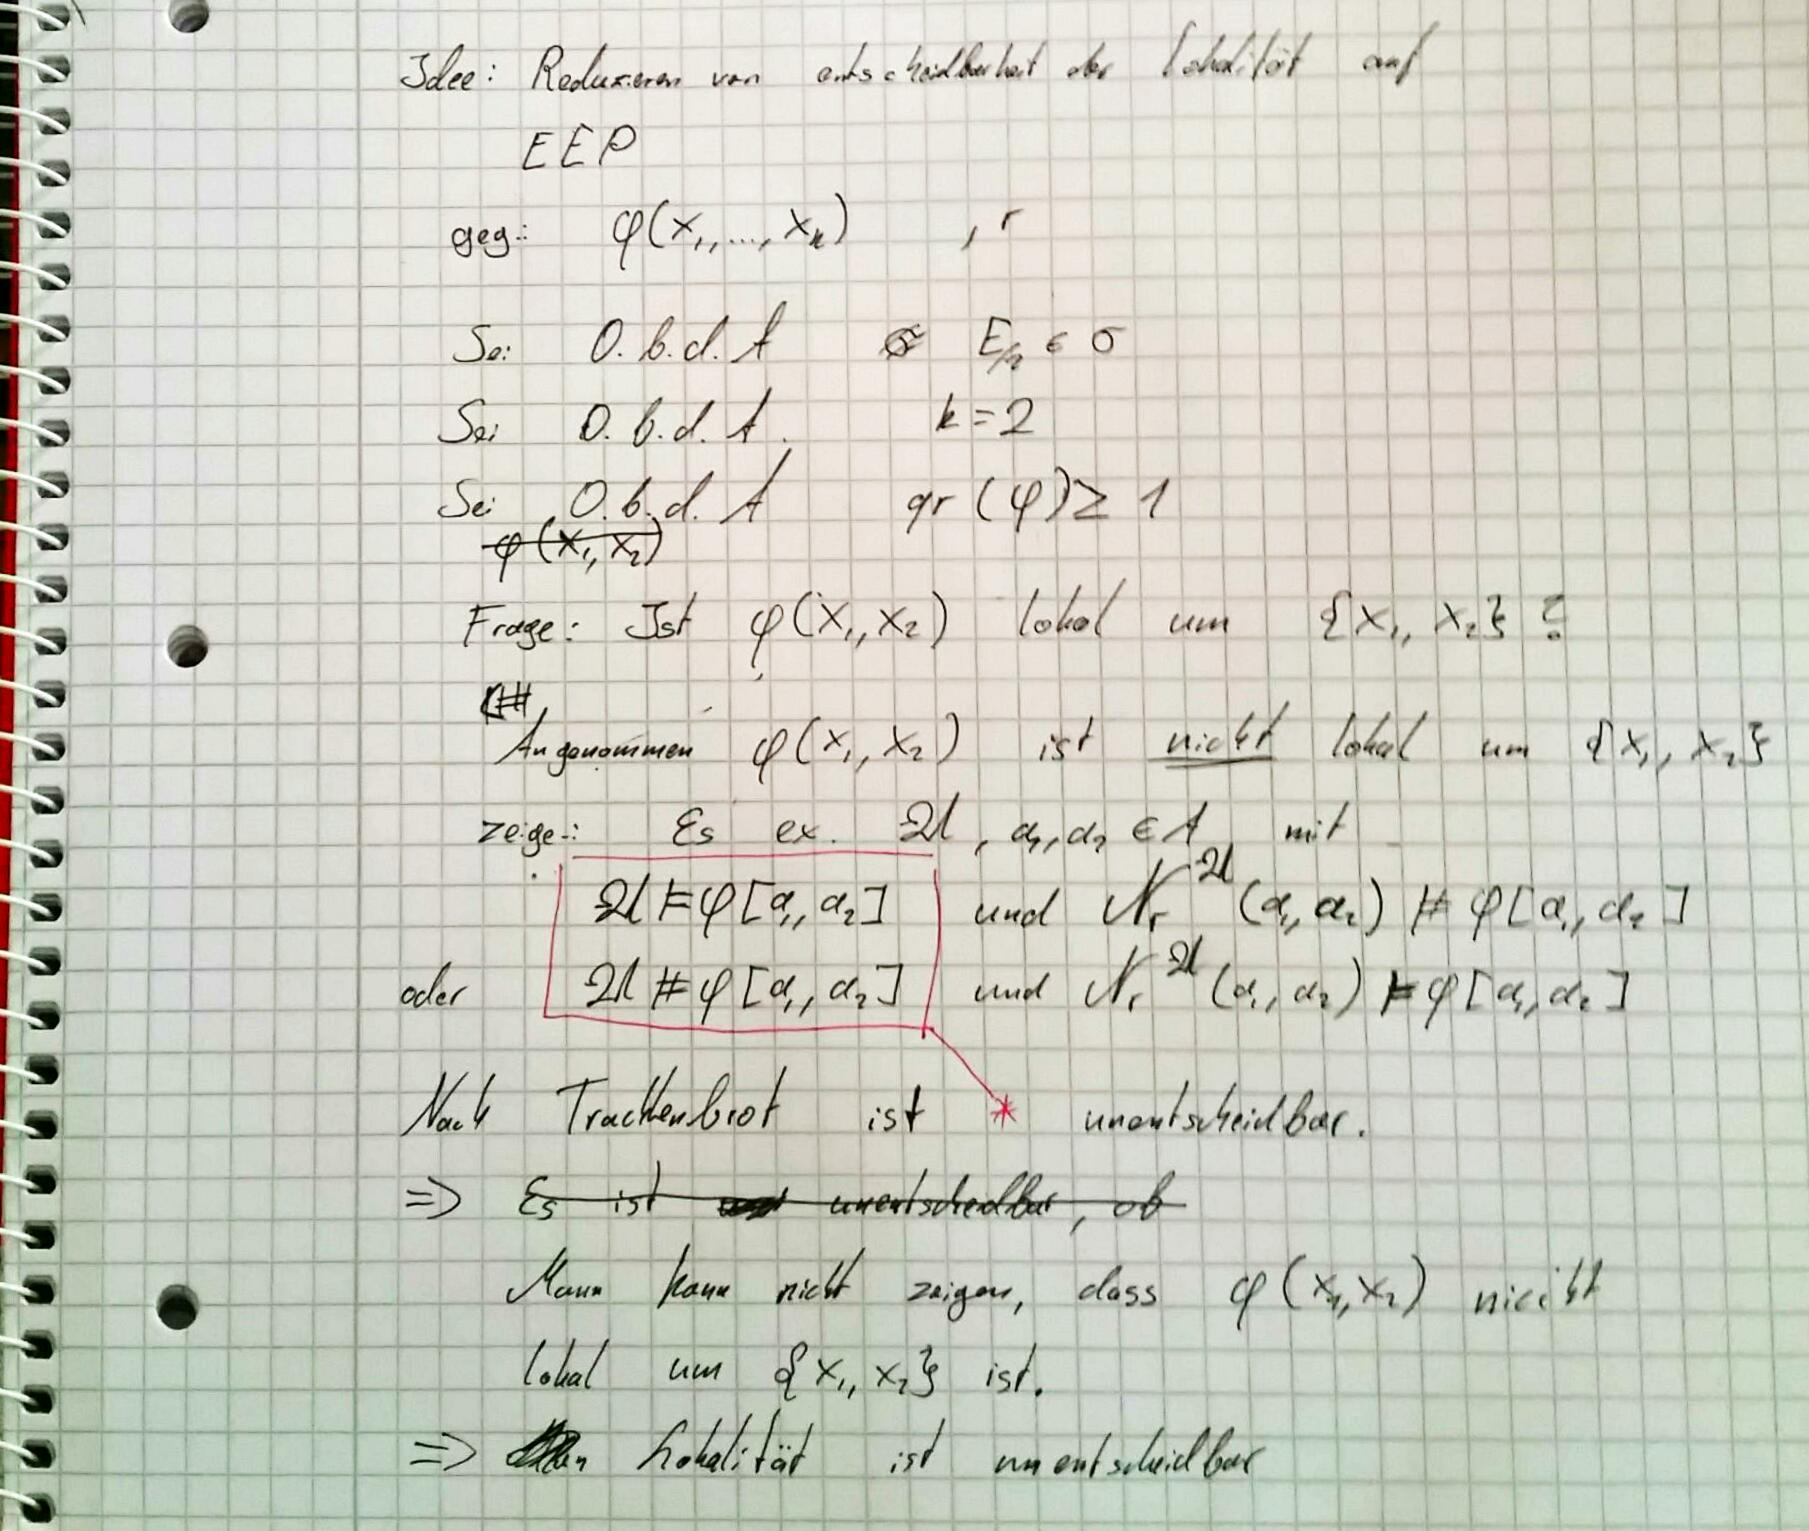
\includegraphics[width=0.8\textwidth]{A3.jpg}
 \caption{}
 \label{}
\end{figure}

% \begin{proof}
%   \step{<1>1}{ \pflet{ $\phi$ ist atomar. } }
%   \step{<1>2}{ $\phi$ ist lokal um $frei(\phi)$ }
%   \step{<1>3} { \pflet{ $\phi$ ist lokal um $frei(\phi)$ } }
%   \step{<1>4} { 
%     \begin{proof}
%       \pf $\neg \phi$ ist lokal um $frei(\phi)$
%       \step{<2>1} {$\mathfrak{A}\models \neg \varphi [\bar a]$}
%       \step{<2>2} {$\mathfrak{A}\nvDash \varphi [\bar a]$}
%       \step{<2>3} {$\mathcal{N}_r^\mathfrak{A}(\bar a)\not\models \varphi [\bar a]$}
%       \step{<2>4} {$\mathcal{N}_r^\mathfrak{A}(\bar a)\models \neg \varphi [\bar a]$}
%       \qedstep Def. r-lokalität
%     \end{proof}
%   }
%   \step{<1>5} {\pflet{ $\phi_1,\phi_2$ sind lokal um jeweils $frei(\phi_1), frei(\phi_2)$ }}
%   \step{<1>6} {
%     \begin{proof}
%       \pf  $\phi_1 \land \phi_2$ sind lokal um $frei(\phi_1) \cup frei(\phi_2)$
%       \step{<2>1} {\pflet{ die benennung von $frei(\varphi_1)$ und $frei(\varphi_2$) ist beliebig. }}
%       \step{<2>2} {\pflet{ $\mathfrak{A}$ beliebig. }}
%       \step{<2>3} {\pflet{ $r := |frei(\varphi_1)\cup frei(\varphi_2)|$ }}
%       \step{<2>4} {\pflet{ $\bar a \in A^r$ }}
%       \step{<2>5} {\pflet{ $\mathfrak{A}\models \varphi_1[\bar a]$ }}
%       \step{<2>6} {\pflet{ $\mathfrak{A}\models \varphi_2[\bar a]$ }}
%       \step{<2>7} {$\mathfrak{A}\models (\varphi_1 \land \varphi_2)[\bar a]$}
%       \step{<2>8} {$\mathcal{N}_r^\mathfrak{A} \models \varphi_1[\bar a]$
%         
%         \pf \stepref{<1>5}, Def. r-lokal }
%       \step{<2>9} {$\mathcal{N}_r^\mathfrak{A} \models \varphi_2[\bar a]$
%         
%         \pf \stepref{<1>5}, Def. r-lokal}
%       \step{<2>10}{$\mathcal{N}_r^\mathfrak{A} \models (\varphi_1 \land \varphi_2)[\bar a]$}
%       \qedstep \pf \stepref{<2>10}, \stepref{<2>7}
%     \end{proof}
%   }
%   \step{} {$\rightarrow, \leftrightarrow, \lor$ lassen sich durch Kombinationen der anderen Fälle darstellen.}
%   \step{} {}
%   
%   
% \end{proof}

\subsection*{Aufgabe 4)}

\begin{figure}[h]
 \centering
 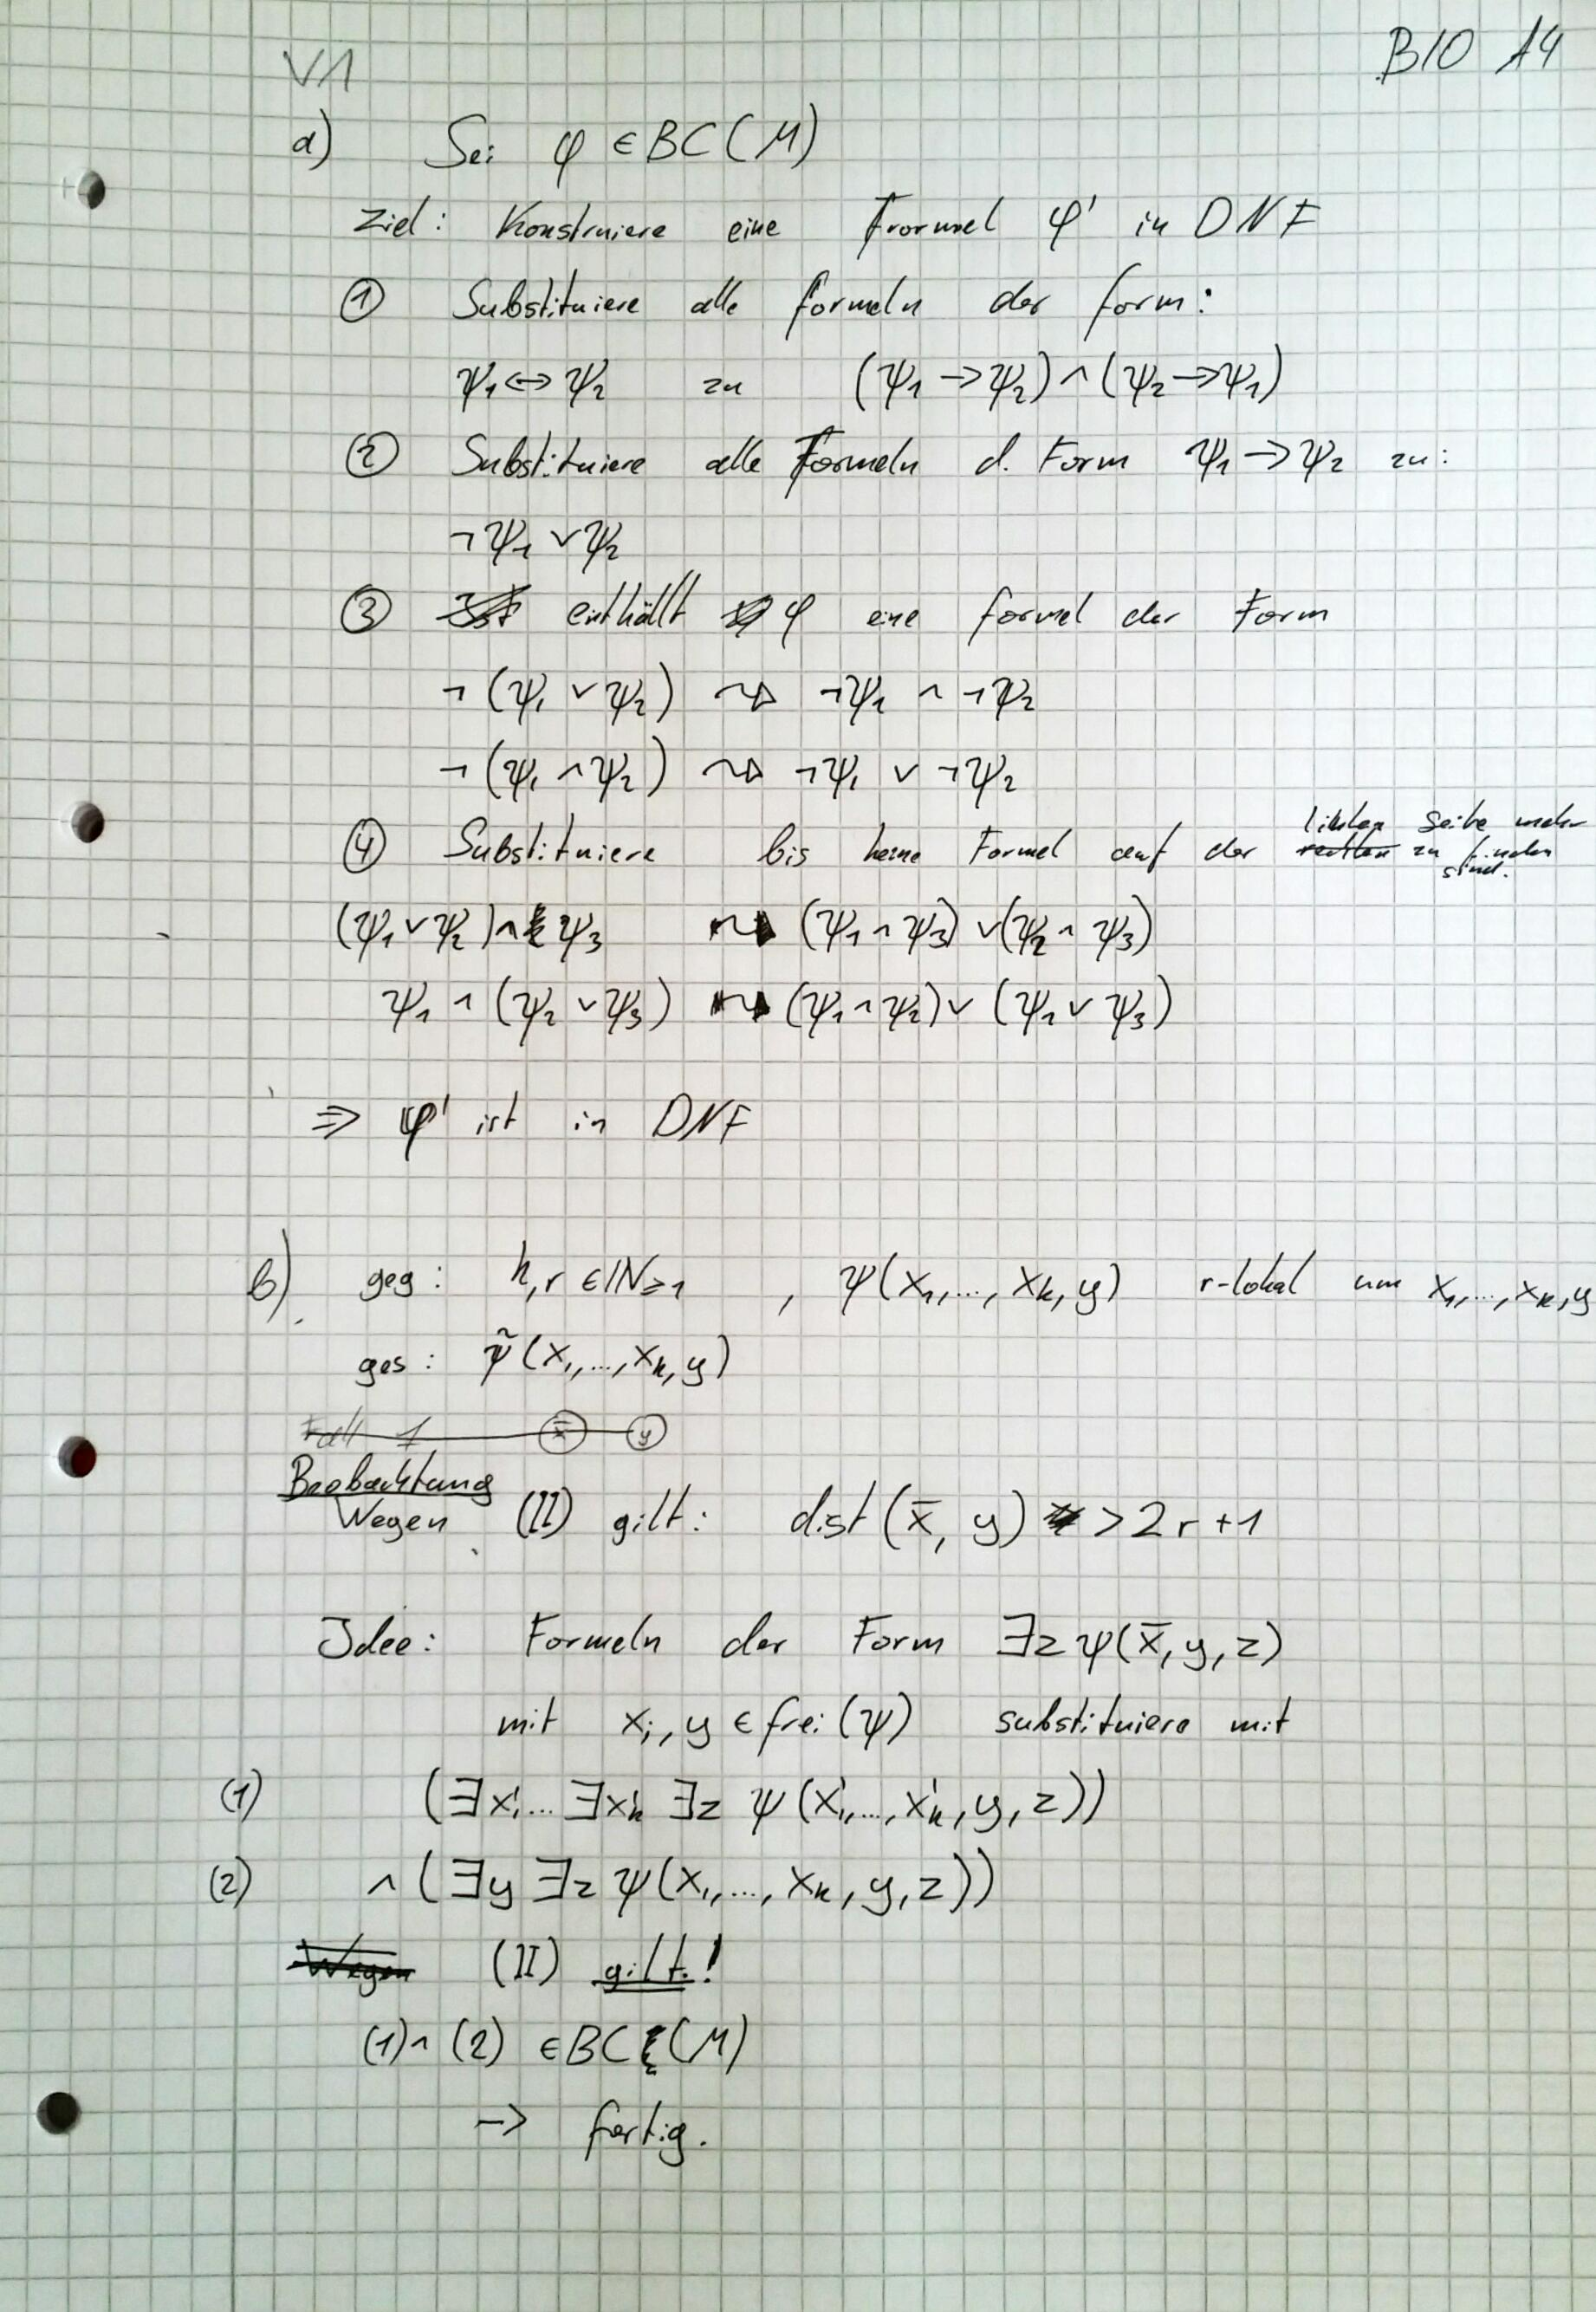
\includegraphics[width=0.8\textwidth]{A4.jpg}
 \caption{}
\end{figure}






\end{document}
